%%% lecture 08 %%%
\documentclass{beamer}
\usepackage[utf8]{inputenc}
\usepackage{algorithm2e, amsmath, amssymb, amsfonts, graphicx, hyperref}
% allow section.equation numbering
\numberwithin{equation}{section}
% use boadilla theme
\usetheme{Boadilla}
% remove navigation symbols
\usenavigationsymbolstemplate{}
% get numbered figure captions
\setbeamertemplate{caption}[numbered]
% changes itemize to circle + other things
\useoutertheme{split}
\useinnertheme{circles}

% command for the title string. change for each lecture
\newcommand{\lecturetitle}{Support Vector Machines}
% allow automatic alert-highlighted references and hyperlinks
\newcommand{\aref}[1]{\alert{\ref{#1}}}
\newcommand{\ahref}[2]{\href{#1}{\alert{#2}}}
% title page stuff. brackets content displayed in footer bar
\title[\lecturetitle]{\lecturetitle}
% metadata. content in brackets is displayed in footer bar
\author[Derek Huang (BAC Advanced Team)]{Derek Huang}
\institute{BAC Advanced Team}
\date{December 31, 2021}

% change "ball" bullet to numbered bullet and section title for section
\setbeamertemplate{section in toc}{\inserttocsectionnumber.~\inserttocsection}
% change ball to gray square (copied from stackoverflow; \par needed for break)
\setbeamertemplate{subsection in toc}{        
    \hspace{1.2em}{\color{gray}\rule[0.3ex]{3pt}{3pt}}~\inserttocsubsection\par
}
% use default enumeration scheme
\setbeamertemplate{enumerate items}[default]
% required line that fixes the problem of \mathbf, \bf not working in beamer
% for later (post-2019) TeX Live installations. see the issue on GitHub:
% https://github.com/josephwright/beamer/issues/630
\DeclareFontShape{OT1}{cmss}{b}{n}{<->ssub * cmss/bx/n}{}

\begin{document}

% title slide
\begin{frame}
    \titlepage
    \centering
    % relative path may need to be updated depending on .tex file location
    
\includegraphics[scale=0.1]{../bac_logo1.png}
\end{frame}

% table of contents slide
\begin{frame}{Overview}
    \tableofcontents
\end{frame}


\section{Separating hyperplanes}

\subsection{Hyperplanes and halfspaces}

\begin{frame}{Motivation}
    \begin{itemize}
        \item
        We saw that logistic regression, LDA/QDA, and na\"{i}ve Bayes
        provide probabilistic models of [class-]conditional distributions.

        \item
        Suppose we have disjoint convex sets $ A, B \subset \mathbb{R}^d $.
        There are several ways to draw a distribution-free ``line''
        (hyperplane) between them.

        \item
        Intuitively, the optimal hyperplane is furthest away from both
        $ A, B $. How can solve the resulting optimization problem?

        \item
        How do we define ``furthest away'' in this context?
    \end{itemize}
\end{frame}

\begin{frame}{Hyperplanes and halfspaces}
    \begin{itemize}
        \item
        \textit{Definition.} A \textit{hyperplane} in $ \mathbb{R}^d $ with
        \textit{normal vector} $ \mathbf{a} \in \mathbb{R}^d $ is the affine
        set
        $ \{\mathbf{x} \in \mathbb{R}^d : \mathbf{a}^\top\mathbf{x} = b \} $,
        where $ \mathbf{a} \ne \mathbf{0} $, $ b \in \mathbb{R} $
        \cite{bv_convex_opt}.

        \item
        A hyperplane is the solution set for a nontrivial linear equation with
        a \textit{normal vector} $ \mathbf{a} $, which in 2D is orthogonal
        to the plane.

        \begin{figure}
            \centering
            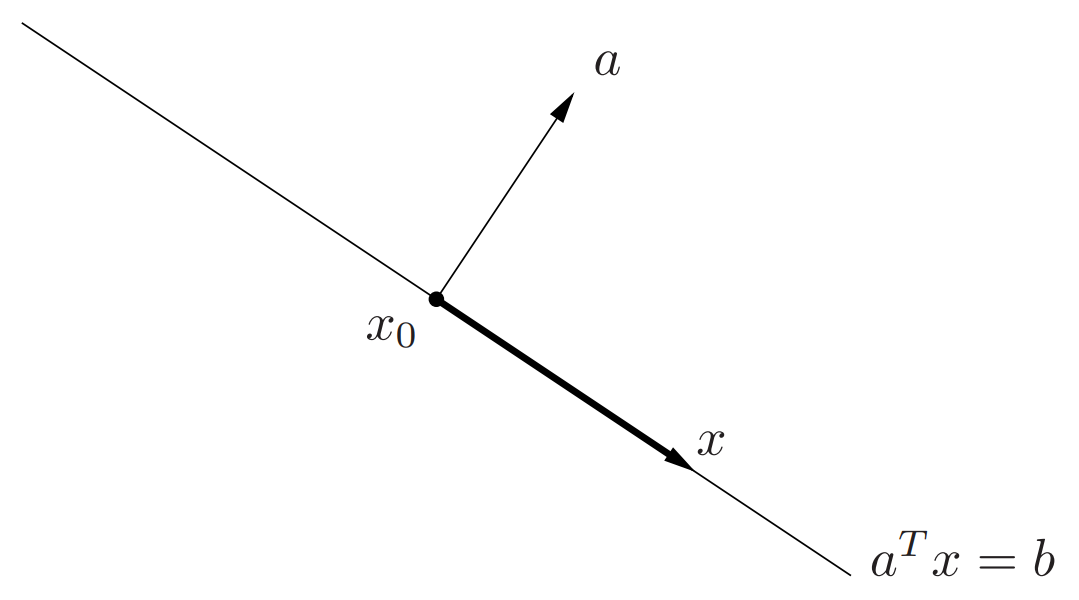
\includegraphics[scale=0.2]{hyperplane.png}
            \vspace{-5 pt}
            \caption{
                A hyperplane with normal vector $ \mathbf{a} \in
                \mathbb{R}^2 $. Note $ \mathbf{a}^\top(\mathbf{x} -
                \mathbf{x}_0) = 0 $\footnote{
                    Figure 2.6 from Boyd and Vandenberghe's
                    \textit{Convex Optimization}.                
                }.
            }
            \label{fig:hyperplane}
            \vspace{-5 pt}
        \end{figure}

        \item
        As seen in Figure \aref{fig:hyperplane}, for hyperplane
        $ L \triangleq \{\mathbf{x} \in \mathbb{R}^d :
        \mathbf{a}^\top\mathbf{x} = b \} $,
        $ \forall \mathbf{x}, \mathbf{y} \in L $,
        $ \mathbf{a}^\top(\mathbf{x} - \mathbf{y}) = 0 \Rightarrow \mathbf{a} $
        is orthogonal to vectors parallel to $ L $.
    \end{itemize}

    % spacing for footnote
    \medskip
\end{frame}

\begin{frame}{Hyperplanes and halfspaces}
    \begin{itemize}
        \item
        \textit{Definition.} A \textit{closed halfspace} in $ \mathbb{R}^d $
        with normal vector $ \mathbf{a} \in \mathbb{R}^d $ is a set of the form
        $ \{\mathbf{x} \in \mathbb{R}^d : \mathbf{a}^\top\mathbf{x} \le b\} $
        or $ \{\mathbf{x} \in \mathbb{R}^d : \mathbf{a}^\top\mathbf{x} \ge
        b\} $ \cite{bv_convex_opt}. If we use strict inequalities, the sets
        are \textit{open halfspaces}.

        \item
        By setting $ b $ to $ -b $, we can equivalently define hyperplanes
        with $ \mathbf{a}^\top\mathbf{x} + b = 0 $ and closed halfspaces with
        $ \mathbf{a}^\top\mathbf{x} + b \le 0 $,
        $ \mathbf{a}^\top\mathbf{x} + b \ge 0 $.

        \item
        Note that $ \forall \mathbf{x}' \in \mathbb{R}^d $, given hyperplane
        $ L \triangleq \{\mathbf{x} \in \mathbb{R}^d :
        \mathbf{w}^\top\mathbf{x} + b = 0 \} $,
        $ \frac{1}{\Vert\mathbf{w}\Vert_2}
        \big(\mathbf{w}^\top\mathbf{x}' + b\big) $ is the signed distance of
        $ \mathbf{x}' $ from $ L $ \cite{esl}.

        \item
        Therefore, $ \mathbf{w}^\top\mathbf{x}' + b \ne 0 \Rightarrow
        \mathbf{x}' $ belongs in one of the open halfspaces defined by $ L $,
        which naturally induces the two-class classification rule
        \begin{equation} \label{eq:svm_classifier}
            G(\mathbf{x}) \triangleq \operatorname{sgn}\big(
                \mathbf{w}^\top\mathbf{x} + b
            \big)
        \end{equation}

        \item
        That is, we label points in $ \{\mathbf{x} \in \mathbb{R}^d :
        \mathbf{w}^\top\mathbf{x} + b > 0\} $ with $ 1 $ and label points in
        $ \{\mathbf{x} \in \mathbb{R}^d : \mathbf{w}^\top\mathbf{x} + b < 0\} $
        with $ -1 $.
    \end{itemize}
\end{frame}

\subsection{Optimal separating hyperplanes}

\begin{frame}{Optimal separating hyperplanes}
    \begin{itemize}
        \item
        Now consider the training data $ \mathcal{D} \triangleq
        \{(\mathbf{x}_1, y_1), \ldots (\mathbf{x}_N, y_N)\} $, where $ \forall
        k \in \{1, \ldots N\} $, $ \mathbf{x}_k \in \mathbb{R}^d $,
        $ y_k \in \{-1, 1\} $.

        \item        
        Furthermore, suppose $ \mathcal{X}_\mathcal{D}^+ \triangleq
        \{\mathbf{x} \in \mathbb{R}^d : (\mathbf{x}, y) \in \mathcal{D},
        y = 1\} $ and $ \mathcal{X}_\mathcal{D}^- \triangleq
        \{\mathbf{x} \in \mathbb{R}^d : (\mathbf{x}, y) \in \mathcal{D},
        y = -1\} $ are linearly separable\footnote{
            In other words, $ \forall (\mathbf{x}, y) \in \mathcal{D} $,
            the scaled unsigned distance
            $ y(\mathbf{w}^\top\mathbf{x} + b) > 0 $.
        }.

        \item
        We thus know $ \exists \{\mathbf{x}' \in \mathbb{R}^d :
        \mathbf{w}^\top\mathbf{x}' + b = 0\} $ s.t. $ \forall (\mathbf{x}, y)
        \in \mathcal{D} $, $ y = G(\mathbf{x}) $, where $ G $ is the
        classification rule defined in (\aref{eq:svm_classifier})\footnote{
            When $ \mathcal{X}_\mathcal{D}^+, \mathcal{X}_\mathcal{D}^- $ are
            convex, the separating hyperplane theorem guarantees existence
            of the separating hyperplane \cite{bv_convex_opt}. Sadly,
            finite sets are by definition nonconvex.
        }.

        \item
        Sadly, the problem of finding \alert{any} separating hyperplane has
        many solutions. However, consider the hyperplane with
        $ \tilde{\mathbf{w}} \in \mathbb{R}^d $,
        $ \Vert\tilde{\mathbf{w}}\Vert_2 = 1 $, $ \tilde{b} \in \mathbb{R} $
        s.t. $ \forall (\mathbf{x}, y) \in \mathcal{D} $,
        $ y\big(\tilde{\mathbf{w}}^\top\mathbf{x} + \tilde{b}\big) \ge M $,
        $ M \in (0, \infty) $ maximized.

        \item
        The $ \tilde{\mathbf{w}}, \tilde{b} $ hyperplane is the \alert{unique}
        \textit{optimal separating hyperplane} due to Vapnik that maximizes
        the quantity $ 2M $, the eponymous \textit{margin}.
    \end{itemize}

    % realign text given footnotes
    \medskip
\end{frame}

\begin{frame}{Optimal separating hyperplanes}
    \begin{itemize}
        \item
        Let $ \mathbf{X} \triangleq [ \ \mathbf{x}_1 \ \ldots \
        \mathbf{x}_N \ ]^\top \in \mathbb{R}^{N \times d} $,
        $ \mathbf{y} \triangleq [ \ y_1 \ \ldots \ y_N \ ]^\top \in
        \{-1, 1\}^N $. Also, let $ \mathbf{Z} \triangleq [ \ y_1\mathbf{x}_1 \
        \ldots \ y_N\mathbf{x}_N \ ]^\top \in \mathbb{R}^{N \times d} $,
        the ``signed'' data matrix.

        \item
        The margin maximization problem can be concisely written as\footnote{
            When feasible, (\aref{eq:max_margin_orig}) has a global solution
            as it is a convex problem.
        }
        \begin{equation} \label{eq:max_margin_orig}
            \begin{array}{ll}
                \displaystyle\max_{\mathbf{w}, b, M} & M \\
                \text{s.t.} &
                \mathbf{Z}\mathbf{w} + b\mathbf{y} \succeq M\mathbf{1}
                \succ \mathbf{0} \\
                & \Vert\mathbf{w}\Vert_2 = 1 \\
            \end{array}
        \end{equation}

        \item
        However, if we drop the $ \mathbf{w} $ norm constraint and redefine
        $ b $ as $ b / \Vert\mathbf{w}\Vert_2 $, we can replace the linear
        constraints
        of (\aref{eq:max_margin_orig}) with\footnote{
            The link is clearer if we rewrite (\aref{eq:neo_margin_cons}) as
            $ \frac{1}{\Vert\mathbf{w}\Vert_2}(\mathbf{Zw} + b\mathbf{y})
            \succeq M\mathbf{1} \succ \mathbf{0} $. % gobble whitespace
            % gobble whitespace
            % prevent fraction from getting smushed into bottom border
            \vspace{0.01 pt}
        } \cite{esl}
        \begin{equation} \label{eq:neo_margin_cons}
            \mathbf{Zw} + b\mathbf{y} \succeq M\Vert\mathbf{w}\Vert_2\mathbf{1}
            \succ \mathbf{0}
        \end{equation}
    \end{itemize}
\end{frame}

\begin{frame}{Optimal separating hyperplanes}
    \begin{itemize}
        \item
        Now suppose $ \mathbf{w}^*, b^*, M^* $ satisfy
        (\aref{eq:neo_margin_cons}), i.e. $ \mathbf{Zw}^* + b^*\mathbf{y}
        \succeq M^*\Vert\mathbf{w}^*\Vert_2\mathbf{1} $. Let $ \hat{\kappa}
        \triangleq 1 / M^*\Vert\mathbf{w}^*\Vert_2 $, $ \hat{\mathbf{w}}
        \triangleq \hat{\kappa}\mathbf{w}^* $, $ \hat{b} \triangleq
        \hat{\kappa}b^* $. Note that
        \begin{equation*}
            \mathbf{Z}\hat{\mathbf{w}} + \hat{b}\mathbf{y} =
            \hat{\kappa}(\mathbf{Zw}^* + b^*\mathbf{y}) \succeq
            \hat{\kappa}M^*\Vert\mathbf{w}^*\Vert_2\mathbf{1} = \mathbf{1}
            \succ \mathbf{0}
        \end{equation*}

        \item
        Furthermore, $ \Vert\hat{\mathbf{w}}\Vert_2 =
        \hat{\kappa}\Vert\mathbf{w}^*\Vert_2 = 1 / M^* $. Therefore, since
        $ \hat{\mathbf{w}}, \hat{b} $ clearly satisfy
        (\aref{eq:neo_margin_cons}), we can solve for them instead, i.e. we
        solve\footnote{
            Squaring the norm gives a nice quadratic objective, i.e. with
            identity Hessian.
        }
        \begin{equation} \label{eq:linear_svc_sep}
            \begin{array}{ll}
                \displaystyle\min_{\mathbf{w}, b} &
                \frac{1}{2}\Vert\mathbf{w}\Vert_2^2 \\
                \text{s.t.} & \mathbf{Zw} + b\mathbf{y} \succeq \mathbf{1}
            \end{array}
        \end{equation}
        Here we set $ \Vert\mathbf{w}\Vert_2 = 1 / M $, so minimizing
        $ \Vert\mathbf{w}\Vert_2 $ is a proxy for maximizing the margin $ 2M $
        as is done in (\aref{eq:max_margin_orig}).

        \item
        (\aref{eq:linear_svc_sep}) is readily solvable, as it has a quadratic
        objective and linear constraints, i.e. it is a \alert{convex}
        optimization problem.
    \end{itemize}

    % footnote spacing
    \medskip
\end{frame}

\section{Linear SVMs}

\subsection{Primal formulation}

\begin{frame}{Primal formulation}
    \begin{itemize}
        \item
        In reality, $ \mathcal{X}_\mathcal{D}^+ $,
        $ \mathcal{X}_\mathcal{D}^- $ may not be linearly separable, in which
        case (\aref{eq:max_margin_orig}), (\aref{eq:linear_svc_sep}) are
        infeasible. Fortunately, this problem is easily addressable.

        \item
        Consider modifying (\aref{eq:max_margin_orig}) to allow
        $ y(\mathbf{w}^\top\mathbf{x} + b) < M $ for some $ (\mathbf{x}, y)
        \in \mathcal{D} $, allowing up to $ K \in (0, \infty) $
        misclassifications.

        \item
        Defining $ \xi \succeq \mathbf{0} \in \mathbb{R}^N $, the ``slack''
        vector\footnote{
            From the Karush-Kuhn-Tucker conditions, $ \xi $ does actually
            define slack variables.
        }, one way to express this change is by replacing the linear
        constraints in (\aref{eq:max_margin_orig}) with\footnote{
            Like in (\aref{eq:max_margin_orig}), $ M > 0 $, but since it is
            implied, we don't explicitly state it.
        }
        \begin{equation} \label{eq:slack_margin_cons}
            \begin{split}
                & \mathbf{Zw} + b\mathbf{y} \succeq M(\mathbf{1} - \xi) \\
                & \mathbf{1}^\top\xi \le K
            \end{split}
        \end{equation}

        \item
        Again dropping the $ \Vert\mathbf{w}\Vert_2 = 1 $ constraint and
        redefining $ b $ as $ b / \Vert\mathbf{w}\Vert_2 $, we can rewrite
        the linear constraints in (\aref{eq:slack_margin_cons}) as
        \begin{equation*}
            \mathbf{Zw} + b\mathbf{y} \succeq
            M\Vert\mathbf{w}\Vert_2(\mathbf{1} - \xi)
        \end{equation*}
    \end{itemize}
\end{frame}

\begin{frame}{Primal formulation}
    \begin{itemize}
        \item
        Now suppose $ \mathbf{w}^* $,  $ b^* $, $ M^* $, $ \xi^* $, satisfy
        (\aref{eq:slack_margin_cons}). Again, if we let $ \hat{\kappa}
        \triangleq 1 / M^*\Vert\mathbf{w}\Vert_2 $, $ \hat{\mathbf{w}}
        \triangleq \hat{\kappa}\mathbf{w}^* $, $ \hat{b} \triangleq
        \hat{\kappa}b^* $, we see that
        \begin{equation*}
            \mathbf{Z}\hat{\mathbf{w}} + \hat{b}\mathbf{y} =
            \hat{\kappa}(\mathbf{Zw}^* + b^*\mathbf{y}) \succeq
            \hat{\kappa}M^*\Vert\mathbf{w}^*\Vert_2(\mathbf{1} - \xi^*) =
            \mathbf{1} - \xi^*
        \end{equation*}

        \item
        Again, $ \Vert\hat{\mathbf{w}}\Vert_2 =
        \hat{\kappa}\Vert\mathbf{w}^*\Vert_2 = 1 / M^* $, so we can modify
        (\aref{eq:linear_svc_sep}) into
        \begin{equation} \label{eq:linear_svc_nonsep}
            \begin{array}{ll}
                \displaystyle\min_{\mathbf{w}, b, \xi} &
                \frac{1}{2}\Vert\mathbf{w}\Vert_2^2 \\
                \text{s.t.} & 
                \mathbf{Zw} + b\mathbf{y} \succeq \mathbf{1} - \xi \\
                & \mathbf{1}^\top\xi \le K \\
                & \xi \succeq \mathbf{0}
            \end{array}
        \end{equation}

        \item
        Note that (\aref{eq:slack_margin_cons}) uses $ M(\mathbf{1} - \xi) $
        despite $ M\mathbf{1} - \xi $ seeming more natural as the latter
        results in a nonconvex\footnote{
            The linear constraints of (\aref{eq:linear_svc_nonsep}) would
            become nonconvex constraints.
        } optimization problem \cite{esl}.
    \end{itemize}
\end{frame}

\begin{frame}{Primal formulation}
    \begin{itemize}
        \item
        In practice, (\aref{eq:linear_svc_nonsep}) is not solved
        directly. Instead, we solve a Lagrangian relaxation of
        (\aref{eq:linear_svc_nonsep}), which for $ C \in (0, \infty) $ is
        \begin{equation} \label{eq:linear_svc_primal}
            \begin{array}{ll}
                \displaystyle\min_{\mathbf{w}, b, \xi} &
                \frac{1}{2}\Vert\mathbf{w}\Vert_2^2 + C\mathbf{1}^\top\xi \\
                \text{s.t.} &
                \mathbf{Zw} + b\mathbf{y} \succeq \mathbf{1} - \xi \\
                & \xi \succeq \mathbf{0}
            \end{array}
        \end{equation}
        Canonically, (\aref{eq:linear_svc_primal}) is the optimization
        problem referred to as the \textit{primal problem}, where the
        $ \mathbf{1}^\top\xi \le K $ constraint has been relaxed\footnote{
            From a computing perspective, fewer constraints are
            preferable, \textit{ceteris paribus}.
        }.

        \item
        Here the Lagrange multiplier $ C $ is the tuning parameter, where
        increasing $ C $ corresponds to decreasing $ K $.

        \item
        Since the solution to (\aref{eq:linear_svc_primal}) has $ d + N + 1 $
        terms, compute time is affected by both feature dimension $ d $ and
        training point number $ N $.
    \end{itemize}
\end{frame}

\subsection{Dual formulation}

\begin{frame}{Dual formulation}
    \begin{itemize}
        \item
        However, by applying some convex optimization theory, we can finesse
        the effect the feature dimension $ d $ has on compute time.

        \item
        Define parameter vector $ \mathbf{x} \in \mathbb{R}^{d + N + 1} $,
        Lagrangian [inequality] multipliers $ \lambda \in \mathbb{R}^{2N} $,
        and block matrices for (\aref{eq:linear_svc_primal})
        s.t. for $ \alpha, \beta \in \mathbb{R}^N $,
        \begin{equation} \label{eq:block_defs}
            \begin{array}{cc}
                \mathbf{x} \triangleq
                \begin{bmatrix}
                    \ \mathbf{w} \ \\
                    \ b \ \\
                    \ \xi \
                \end{bmatrix} &
	            \mathbf{D} \triangleq \begin{bmatrix}
	                \ \mathbf{I}_d & \mathbf{0}_{d \times (N + 1)} \ \\
	                \ \mathbf{0}_{(N + 1) \times d} &
	                \mathbf{0}_{(N + 1) \times (N + 1)} \
	            \end{bmatrix} \\ \\
	            \lambda \triangleq
                \begin{bmatrix} \ \alpha \ \\ \ \beta \ \end{bmatrix} &
	            \mathbf{Q} \triangleq \begin{bmatrix}
                    \ \mathbf{Z} & \mathbf{y} & \mathbf{I}_N \ \\
                    \ \mathbf{0}_{N \times d} & \mathbf{0}_N & \mathbf{I}_N \
	            \end{bmatrix}
            \end{array}
        \end{equation}

        \item
        Now let $ \mathcal{L} : \mathbb{R}^{d + N + 1} \times \mathbb{R}^{2N}
        \rightarrow \mathbb{R} $ be the Lagrangian for
        (\aref{eq:linear_svc_primal}), where
        \begin{equation} \label{eq:linear_svc_lagrangian}
            \mathcal{L}(\mathbf{x}, \lambda) \triangleq
            \frac{1}{2}\mathbf{x}^\top\mathbf{D}\mathbf{x} + \begin{bmatrix}
                \ \mathbf{0}_{d + 1}^\top & C\mathbf{1}_N^\top \
            \end{bmatrix}\mathbf{x} +
            \lambda^\top\left(
                \begin{bmatrix}
                    \ \mathbf{1}_N \ \\ \ \mathbf{0}_N \
                \end{bmatrix} -
                \mathbf{Q}\mathbf{x}
            \right)
        \end{equation}
    \end{itemize}
\end{frame}

\begin{frame}{Dual formulation}
    \begin{itemize}
        \item
        Since $ \mathcal{L} $ is convex in $ \mathbf{x} $, for any
        fixed $ \lambda $, $ \mathbf{x}_\lambda \triangleq
        \arg\min_\mathbf{x}\mathcal{L}(\mathbf{x}, \lambda) $ is
        s.t.\footnote{
            Of course, we know $ \nabla_\mathbf{x}\mathcal{L}(
            \mathbf{x}_\lambda, \lambda) \triangleq \mathbf{Dx}_\lambda +            
            \begin{bmatrix}
                \ \mathbf{0}_{d + 1} \ \\ \ C\mathbf{1}_N \
            \end{bmatrix} - \mathbf{Q}^\top\lambda = \mathbf{0}_{d + N + 1} $.
            % if omitted, inline math is clipped
            \vspace{0 pt}
        }
        \begin{equation} \label{eq:linear_dual_system}
            \mathbf{Dx}_\lambda + \begin{bmatrix}
                \ \mathbf{0}_{d + 1} \ \\ \ C\mathbf{1}_N \
            \end{bmatrix} = \mathbf{Q}^\top\lambda
        \end{equation}

        \item
        Recalling (\aref{eq:block_defs}), we can rewrite
        (\aref{eq:linear_dual_system}) as the block system
        \begin{equation} \label{eq:linear_dual_eqs}
            \begin{bmatrix}
                \ \mathbf{w}_\lambda \ \\ \ 0 \ \\ \ C\mathbf{1} \
            \end{bmatrix} = \begin{bmatrix}
                \ \mathbf{Z}^\top\alpha \ \\
                \ \alpha^\top\mathbf{y} \ \\
                \ \alpha + \beta \
            \end{bmatrix}
        \end{equation}

        \item
        Using (\aref{eq:linear_svc_lagrangian}),
        (\aref{eq:linear_dual_system}), (\aref{eq:linear_dual_eqs}), noting
        $ \mathbf{x}_\lambda^\top\mathbf{Dx}_\lambda =
        \mathbf{w}_\lambda^\top\mathbf{w}_\lambda $, we see that
        \begin{equation} \label{eq:linear_svc_dual_func}
            \mathcal{L}(\mathbf{x}_\lambda, \lambda) = \lambda^\top
            \begin{bmatrix}
                \ \mathbf{1}_N \ \\ \ \mathbf{0}_N \
            \end{bmatrix} -
            \frac{1}{2}\mathbf{x}_\lambda^\top\mathbf{Dx}_\lambda =
            \mathbf{1}^\top\alpha -
            \frac{1}{2}\alpha^\top\mathbf{ZZ}^\top\alpha
        \end{equation}
    \end{itemize}
\end{frame}

\begin{frame}{Dual formulation}
    \begin{itemize}
        \item
        Noting that $ \mathcal{L}(\mathbf{x}_\lambda, \lambda) \triangleq
        \inf_\mathbf{x}\{\mathcal{L}(\mathbf{x}, \lambda)\} $, i.e. the dual
        of the objective in (\aref{eq:linear_svc_primal}),
        (\aref{eq:linear_svc_dual_func}) implies we can express the dual
        only through $ \alpha \in \mathbb{R}^N $.

        \item
        Thus, from (\aref{eq:linear_dual_eqs}),
        (\aref{eq:linear_svc_dual_func}), we can express the dual of the
        primal (\aref{eq:linear_svc_primal}) as
        \begin{equation} \label{eq:linear_svc_dual}
            \begin{array}{ll}
                \displaystyle\max_\alpha & \mathbf{1}^\top\alpha -
                \frac{1}{2}\alpha^\top\mathbf{ZZ}^\top\alpha \\
                \text{s.t.} & \alpha^\top\mathbf{y} = 0 \\
                & \mathbf{0} \preceq \alpha \preceq C\mathbf{1}
            \end{array}
        \end{equation}
        Here the constraints are due to (\aref{eq:linear_dual_eqs}) and the
        dual constraint $ \lambda \succeq \mathbf{0} $, as from
        (\aref{eq:linear_dual_eqs}), $ \alpha = C\mathbf{1} - \beta $, so
        with $ \alpha, \beta \succeq \mathbf{0} $, we have 
        $ \mathbf{0} \preceq \alpha \preceq C\mathbf{1} $.

        \item
        Note how the solution to (\aref{eq:linear_svc_dual}) has $ N $ terms
        compared to $ d + N + 1 $ terms for (\aref{eq:linear_svc_primal}), so
        we have finessed the effect of feature dimension.

        \item
        Solving (\aref{eq:linear_svc_dual}) is preferred, as it has a
        lower-dimension solution independent of feature dimension and
        simpler constraints than (\aref{eq:linear_svc_primal}).
    \end{itemize}
\end{frame}

\section{Dual SVMs}

\subsection{Dual to primal}

\begin{frame}{Dual to primal}
    \begin{itemize}
        \item
        However, after solving (\aref{eq:linear_svc_dual}), we must recover
        the primal solution to classify new points, so we use some more
        optimization theory.

        \item
        Since (\aref{eq:linear_svc_primal}) convex with only linear
        constraints, $ \mathbb{R}^{d + N + 1} $ open\footnote{
            Using any valid metric on $ \mathbb{R}^{d + N + 1} $, this is
            trivial to show.
        }, and
        $ (\mathbf{0}, 0, \mathbf{1}) $ feasible, strong duality
        holds\footnote{
            Slater's condition reduces to feasibility in this case.
        } for (\aref{eq:linear_svc_primal})
        \cite{bv_convex_opt}.

        \item
        Strong duality $ \Rightarrow $ the primal optimal $ \hat{\mathbf{w}}, \hat{b}, \hat{\xi} $ and dual optimal $ \hat{\lambda} $ solutions exhibit complementary slackness. Thus, $ \forall k \in \{1, \ldots N\} $,
        \begin{equation}
            \begin{split}
            \hat{\alpha}_k\big(1 - \hat{\xi}_k - y_k\big(\mathbf{x}_k^\top\hat{\mathbf{w}} + \hat{b}\big)\big) & = 0 \\
                \hat{\beta}_k\hat{\xi}_k & = 0
            \end{split}
        \end{equation}

        \item
        Since $ \hat{\beta}_k > 0 \Leftrightarrow \hat{\xi}_k = 0 $,  
    \end{itemize}
\end{frame}

% BibTeX slide for references. should use either acm or ieeetr style
\begin{frame}{References}
    \bibliographystyle{acm}
    % relative path may need to be updated depending on .tex file location
    \bibliography{../master_bib}
\end{frame}

\end{document}